\subchapter{Application development and application
debugging}{Objective: compile an application against a Buildroot
build space and debug it remotely.}

\section{Setup}

We will continue to use the same root filesystem.

Our goal is to compile and debug our own {\em MPD} client. This client
will be driven by the Nunckuk to switch between audio tracks, and to
adjust the playback volume.

However, this client will be used together with \code{mpc}, as it won't
be able to create the playlist and start the playback. It will just be
used to control the volume and switch between songs. So, you run to
run \code{mpc} commands first before trying the new client:

\begin{bashinput}
mpc update
mpc add /
mpc pause
\end{bashinput}

We will use the new client to resume playback.

\section{Compile your own application}

Go to the \code{$HOME/__SESSION_NAME__-labs/appdev} directory.

In the lab directory the file \code{nunchuk-mpd-client.c} contains an
application which implements a simple MPD client based on the
{\em \href{https://musicpd.org/libs/libmpdclient/}{libmpdclient}} library.
As {\em mpc} is also based on this library, Buildroot already compiled
it and added it to our root filesystem. What's special in this
application is that it allows to drive music playback through our
Nunchuk.

Buildroot has generated toolchain wrappers in
\code{output/host/bin}, which make it easier to use the toolchain,
since these wrappers pass some mandatory flags (especially the
\code{--sysroot} {\em gcc} flag, which tells {\em gcc} where to look
for the headers and libraries). This way, we can compile our application
outside of Buildroot, as often as we want.

Let's add this directory to our \code{PATH}:

\small
\begin{bashinput}
$ export PATH=$HOME/__SESSION_NAME__-labs/integration/buildroot-2022.02.X/output/host/bin:$PATH
\end{bashinput}
\normalsize

Let's try to compile the application:

\bashcmd{$ arm-linux-gcc -o nunchuk-mpd-client nunchuk-mpd-client.c}

The compiler complains about undefined references to some symbols in
{\em libmpdclient}. This is normal, since we didn't tell the compiler
to link with this library. So let's use \code{pkg-config} to query the
{\em pkg-config} database about the location of the header files and
the list of libraries needed to build an application against
{\em libmpdclient}\footnote{Again, \code{output/host/bin} has a special
\code{pkg-config} that automatically knows where to look, so it
already knows the right paths to find \code{.pc} files and their
sysroot.}:

\begin{bashinput}
$ arm-linux-gcc -o nunchuk-mpd-client nunchuk-mpd-client.c \
$(pkg-config --libs --cflags libmpdclient)
\end{bashinput}

Strip the \code{nunchuk-mpd-client} program, and copy
the resulting binary to the \code{/root} directory of the root
filesystem.

Back to target system, try to run the program:

\begin{bashinput}
# /root/nunchuk-mpd-client
ERROR: didn't manage to find the Nunchuk device in /dev/input. Is the Nunchuk driver loaded?
\end{bashinput}

\section{Using strace}

Let's run the program through the \code{strace} command to find out why
this happens.

You should see that it's trying to access files that don't exist.
Once you've found what's wrong, fix the code (or ask your instructor for
help if needed), then rebuild the program and run it again:

\begin{bashinput}
# /root/nunchuk-mpd-client
ERROR: didn't manage to find the Nunchuk device in /dev/input. Is the Nunchuk driver loaded?
\end{bashinput}

Ouch, same problem again!

You can run the program again through \code{strace}, and check that the
right paths are now accessed, but the cause of the issue won't be easy
to find.

\section{Using ltrace}

Let's run the program through \code{ltrace} now. We will be able to see
not only the system calls, but also the shared library calls.

Take your time to study the \code{ltrace} output. That's interesting
information! Back to our issue, the last lines of output should make the
issue pretty obvious.

Fix the bug in the code, recompile the program, strip it, copy it to
the target and start it again.

You should now be able to use the new client, driving the server
through the following Nunchuk inputs:

\begin{itemize}
   \item Joystick up: volume up 5\%
   \item Joystick down: volume down 5\%
   \item Joystick left: previous song
   \item Joystick right: next song
   \item Z (big) button: pause / play
   \item C (small) button: quit client
\end{itemize}

Have fun with the new client. You'll just realize that quitting
causes the program to crash with a segmentation fault. Let's debug this
too.

\section{Using gdbserver from the command line}

We are going to use \code{gdbserver} to understand why the program
segfaults.

Compile \code{nunchuk-mpd-client.c} again with the \code{-g} (\code{g}
means {\em gdb}) option to include debugging symbols. This time, just
keep it on your workstation, as you already have the version without
debugging symbols on your target.

Then, on the target side, run the program under \code{gdbserver}.
\code{gdbserver} will listen on a TCP port for a connection from
\code{gdb} on the host, and will control the execution of
\code{nunchuk-mpd-client} according to the \code{gdb} commands:

\ubootcmd{=> gdbserver localhost:2345 /root/nunchuk-mpd-client}

On the host side, run \code{arm-linux-gdb} (also found in your toolchain):
\bashcmd{$ arm-linux-gdb nunchuk-mpd-client}

\code{gdb} starts and loads the debugging information from the
\code{nunchuk-mpd-client} binary (in the \code{appdev} directory)
which has been compiled with \code{-g}.

Then, we need to tell where to find our libraries, since they are not
present in the default \code{/lib} and \code{/usr/lib} directories on
your workstation. This is done by setting the \code{gdb} \code{sysroot}
variable (on one line):

\begin{bashinput}
(gdb) set sysroot /home/<user>/__SESSION_NAME__-labs/debugging/\
    buildroot-2022.02.<n>/output/staging
\end{bashinput}

Of course, replace \code{<user>} by your actual user name.

And tell \code{gdb} to connect to the remote system:
\begin{bashinput}
(gdb) target remote <target-ip-address>:2345
\end{bashinput}

Then, use \code{gdb} as usual to set breakpoints, look at the source
code, run the application step by step, etc.

In our case, we'll just start the program, press the \code{C} button
to quit to cause the the segmentation fault:
\begin{bashinput}
(gdb) continue
\end{bashinput}

After the segmentation fault, you can ask for a backtrace to see
where this happened:
\begin{bashinput}
(gdb) backtrace
\end{bashinput}

This will tell you that the segmentation fault occurred in a function
of the \code{libmpdclient}, called by our program. You will also get
the number of the line in the program which caused this. This should
help you to find the bug in our application.

Once you found it, don't fix it yet. We are going to make further
experiments around this segmentation fault.

\section{Post mortem analysis}

Following the details in the slides, configure your shell on the
target to get a \code{core.xxx} file dumped when you run
\code{nunchuk-mpd-client} again.

Once you have such a file, inspect it with \code{arm-linux-gdb} on
the target, set the \code{sysroot} setting, and then generate
a backtrace to see where the program crashed.

You can even see the value of all variables in the different
function contexts of your program:

\begin{bashinput}
(gdb) bt full
\end{bashinput}

This way, you can have a lot of information about the crash
without running the program through the debugger.

\section{Editing and remote compiling with VS Code}

\subsection{Installing software}

We are going to use Visual Studio Code to do the remote debugging
again, and eventually fix and recompile our program.

The first thing to do is install VS Code. This package is only available
as a {\em snap package}:

\begin{bashinput}
$ sudo snap install --classic code
\end{bashinput}

\subsection{Accessing your board through SSH}

We will use Visual Studio Code to modify and recompile our client
program, and also to update and run the binary on the target.
Of course, we will use a simple solution, as we won't be able to
spend too much time learning about all the possibilities offered
by VS Code.

For our purpose, a good solution is SSH, which allows to copy files
(through the \code{scp} command) and to run remote commands. We already
included the {\em Dropbear} SSH server in our root filesystem.

We just need to implement password-less SSH access, to keep things
simple:

\begin{itemize}
  \item If you don't have an SSH key yet (look at \code{~/.ssh/},
	generate one with the \code{ssh-keygen} command.
	By defaults, this creates two files in \code{~/.ssh/}:
	\code{id_rsa} (private key) and \code{id_rsa.pub} (public key).
  \item Then create the \code{/root/.ssh} directory {\bf on the target}
        and in it, create an \code{authorized_keys} file with the line in
        \code{id_rsa.pub}.
  \item Then, fix permissions on the target, as Dropbear is quite strict
        about them:
        \begin{bashinput}
# chmod go-rwx /root
# chown -R root.root /root
        \end{bashinput}
\end{itemize}

Then, you can test that SSH works without a password:

\begin{bashinput}
ssh root@192.168.0.100
\end{bashinput}

\subsection{Compiling and debugging the program from VS Code}

The \code{appdev} directory already contains a \code{prep-debug.sh}
script and a \code{.vscode} directory with ready made settings for
code editing and for compiling and debugging our application.
Here are these files:

\begin{itemize}
   \item \code{prep-debug.sh}: script to recompile the program,
         copy it to the target through SSH, and start it through the debugger.
         Open this file and update the target IP and path settings if
         necessary.
   \item \code{.vscode/c_cpp_properties.json}: settings for the code editor.
         Modify the paths in this file according to your setup.
   \item \code{.vscode/tasks.json}: definition of a "build" task,
         calling the \code{prep-debug.sh} script.
   \item \code{.vscode/launch.json}: these are the settings for remote
         debugging. Again, open this file, update the paths, and the
	 target IP address if necessary.
\end{itemize}

First, from the \code{appdev} directory, start VS Code:

\begin{bashinput}
$ code
\end{bashinput}

The use \code{File} $\rightarrow$ \code{Open Folder} to open the
\code{appdev} directory.

The first thing to do is to make sure the \code{C/C++} extension from Microsoft
(\code{ms-vscode.cpptools}) is installed. Do this using the
\code{Extensions} vertical tab:

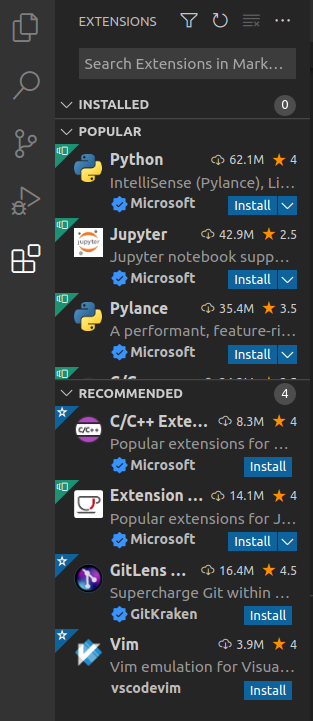
\includegraphics[width=2cm]{labs/sysdev-application-development-and-debugging/vscode-extensions-tab.png}

Then click on the \code{nunchuk-mpd-client.c} file in the left
column to open it in VS Code.

Now, start by compiling your program from VS Code, copying it to the
target, and running it through the debugger by using the
\code{Terminal} $\rightarrow$ \code{Run Build Task...} menu entry.

If anything goes wrong, please report issues to the trainer.

Last but not least, you can start debugging the program by clicking on
the \code{Run and Debug} tab, and then on the \code{gdb (Launch)} at the
top:

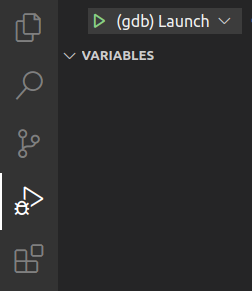
\includegraphics[width=2cm]{labs/sysdev-application-development-and-debugging/vscode-run-debug-tab.png}

In the debug console, you should see that debugging has started. The
bottom line of the interface should turn orange too:

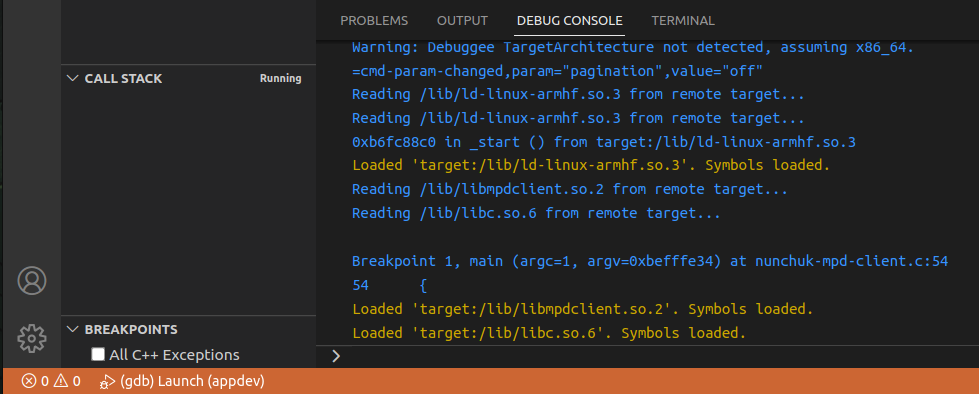
\includegraphics[width=12cm]{labs/sysdev-application-development-and-debugging/vscode-debugging-started.png}

Then, start using the Nunchuk to control playback, and when you try to
quit with the \code{C} button, VS Code should now see the segmentation
fault:

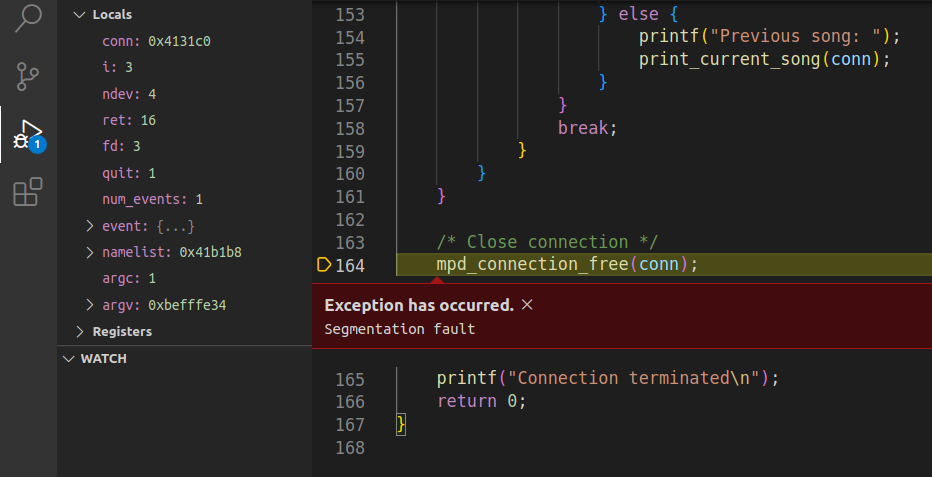
\includegraphics[width=12cm]{labs/sysdev-application-development-and-debugging/vscode-segmentation-fault.png}

You can then look at variables, the call stack, browse the code...

To stop debugging, you should use \code{Run} $\rightarrow$ \code{Stop
Debugging}.

By studing the the code, you should eventually find that what's causing
the segmentation fault is the call to \code{free()} in the test for the
\code{C} button. Remove this line, save the file through the \code{File}
menu (otherwise nothing will change), and then compile and run the
application again. This time, there should be no more segmentation fault
when you hit the \code{C} button.

If you are ahead of time, don't hesitate to spend more time with VS
Code, for example to add breakpoints and execute the program step by
step.

\section{Profiling the application with perf}

Let's make a quick attempt at profiling our application with the
\code{perf} command.

To add \code{perf} to the root filesystem, we have to build it from
kernel sources (see \kdir{tools/perf} in the kernel source code), and
the \code{perf} version has to be in sync with the kernel version.

That's why, to build \code{perf}, Buildroot builds the kernel at the
same time. In our case, we don't have time to integrate the kernel in
the image built by Buildroot, but that's something a real project will
ultimately do.

So, go back to Buildroot's configuration interface and, in the
\code{Kernel} menu:
\begin{itemize}
\item Enable \code{Linux Kernel}
\item Set \code{Kernel version} to \code{Custom version}
\item Set \code{Custom version} to the exact \workingkernel ~version
      you used.
\item Set \code{Kernel configuration} to \code{Using a custom (def)config file})
\item Set \code{Configuration file path} to the full path of your kernel \code{.config} file.
\item In \code{Linux Kernel Tools}, enable \code{perf}
\end{itemize}

Then run \code{make}, and once this is done, update your root
filesystem. This will take time to recompile the kernel again, together
with all its modules. You can start working on the {\em Going further}
section to save time though.

By the way, why didn't we make Buildroot deploy the Linux kernel,
modules and DTB directly to the root filesystem? We would have done that
pretty easily, and you would do this in a real project, if we didn't
have our of tree module.

To build an external kernel module with Buildroot, it would have required
adding a special package for this purpose, but our time is limited.

Once the new root filesystem is ready, you can now run:

\begin{bashinput}
perf record /root/nunchuk-mpd-client
\end{bashinput}

Use your application and leave it when you are done.

This stores profiling data in a \code{perf.data} file. One way to
extract information from it is to run the below command in the same
directory (the one containing \code{perf.data}):

\begin{bashinput}
perf report
\end{bashinput}

See the time spent in various kernel (\code{[k]}) and userspace
(\code{[.]}) functions.

Now, let's profile the whole system. First, make sure that the system is
currently playing audio. Then SSH to your board and run \code{perf top}
(working better through SSH) to see live information about kernel and
userspace functions consuming most CPU time.

This was a very brief start at practising with \code{perf}, which offers
many more possibilities than we could see here.

\section{What to remember}

During this lab, we learned that...

\begin{itemize}
\item It's easy to study the behavior of programs and diagnose issues
  without even having the source code, thanks to \code{strace},
  \code{ltrace} and \code{perf}.

\item You can use \code{perf} as a system wide profiler too.

\item You can leave a small \code{gdbserver} program (about 400 KB) on your target
  that allows to debug target applications, using a standard \code{gdb}
  debugger on the development host, or a graphical IDE such as VS Code.

\item It is fine to strip applications and binaries on the target
  machine, as long as the programs and libraries with debugging
  symbols are available on the development host.

\item Thanks to \code{core} dumps, you can know where a program crashed,
  without having to reproduce the issue by running the program through
  the debugger.
\end{itemize}

\section{Going further: packaging your application with Meson}

Now that our application is ready, the next thing to do is to properly
integrate it into our root filesystem. This is a nice opportunity to see
how to do this with {\em Meson} and leverage Buildroot's
infrastructure to cross-compile {\em Meson} based packages.

Still in the main \code{appdev} directory, create a
\code{nunchuk-mpd-client-1.0} directory and copy the
\code{nunchuk-mpd-client.c} file to it.

In this new directory, all you have to do is create a very simple
\code{meson.build} file:

\begin{verbatim}
project('nunchuk-mpd-client', 'c', version: '1.0')
libmpdclient_dep = dependency('libmpdclient', version: '>= 2.16')
executable('nunchuk-mpd-client', 'nunchuk-mpd-client.c',
           dependencies: libmpdclient_dep, install: true)
\end{verbatim}

Note that \code{install: true} is necessary to get the executable installed
by \code{ninja install}.

Now, the next thing is to add a new package to the Buildroot source
tree:
\begin{itemize}
\item Create a \code{nunchuk-mpd-client} directory under \code{package}.
\item In this directory, create a \code{Config.in} file. You can reuse
      the one from the \code{mpd-mpc} package (the {\em mpc} client)
      which also depends on {\em libmpdclient}.
\item Modify \code{package/Config.in} to source this new file in the
      \code{Audio and video applications} submenu.
\item Last but not least, create the \code{nunchuk-mpd-client.mk} file
      with the following contents:
\begin{verbatim}
################################################################################
#
# nunchuk-mpd-client
#
################################################################################

NUNCHUK_MPD_CLIENT_VERSION = 1.0
NUNCHUK_MPD_CLIENT_SITE = $(HOME)/embedded-linux-labs/appdev/nunchuk-mpd-client-1.0
NUNCHUK_MPD_CLIENT_SITE_METHOD = local
NUNCHUK_MPD_CLIENT_DEPENDENCIES = host-pkgconf libmpdclient

$(eval $(meson-package))
\end{verbatim}
\end{itemize}

All you have to do now is to enable the \code{nunchuk-mpd-client}
package in Buildroot's configuration, run \code{make}, update the root
filesystem and check on the target that
\code{/usr/bin/nunchuk-mpd-client} exists and runs fine.

All this was pretty straightforward, wasn't it? {\em Meson} rocks!

Congratulations, you've reached the end of all our labs. Try to look
back, and see how much experience you've gained in these last days.
